
    \begin{longtable}{cc}
    
\raisebox{6.5em}{\Huge A} &
    				\begin{adjustbox}{max width=0.925\textwidth}
    					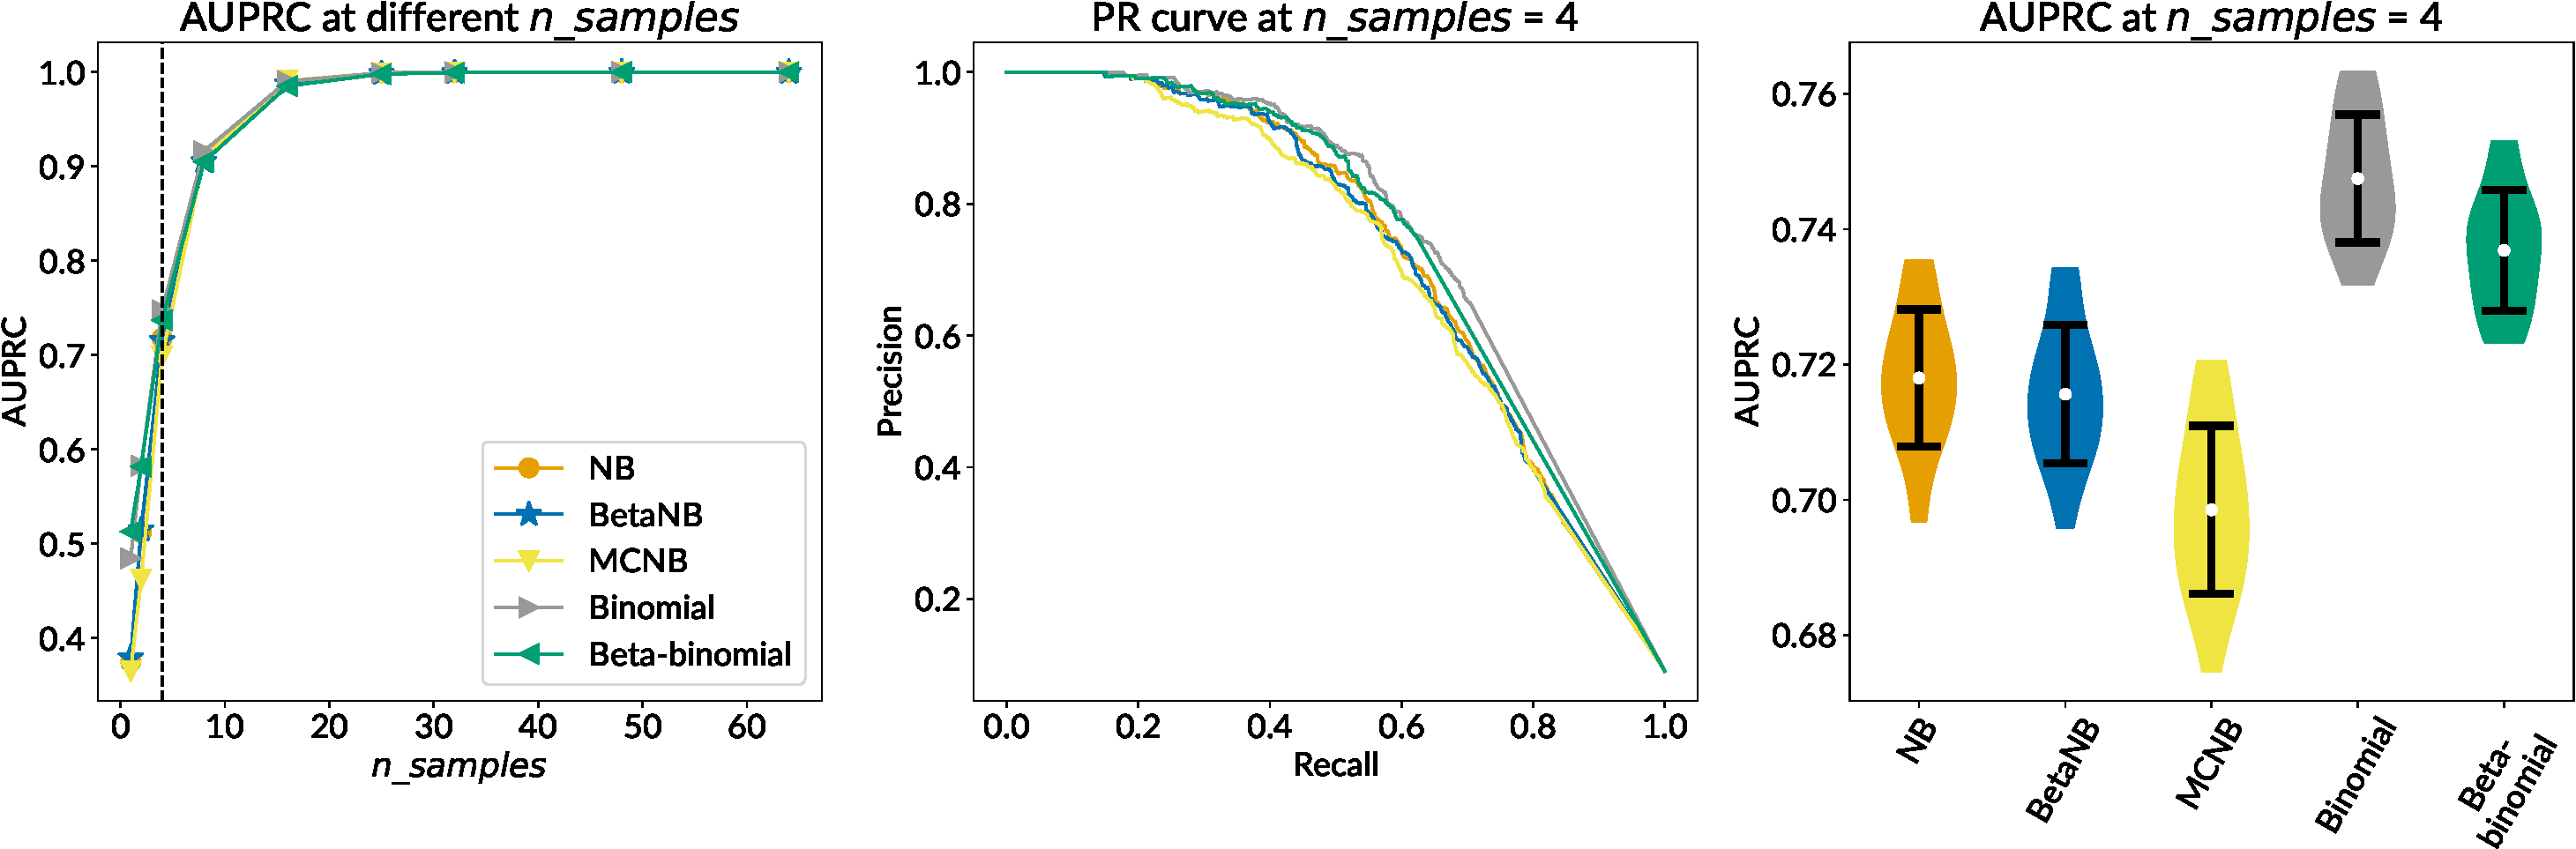
\includegraphics{figures/benchmark/A}
    				\end{adjustbox}
    \\
\raisebox{6.5em}{\Huge B} &
    				\begin{adjustbox}{max width=0.925\textwidth}
    					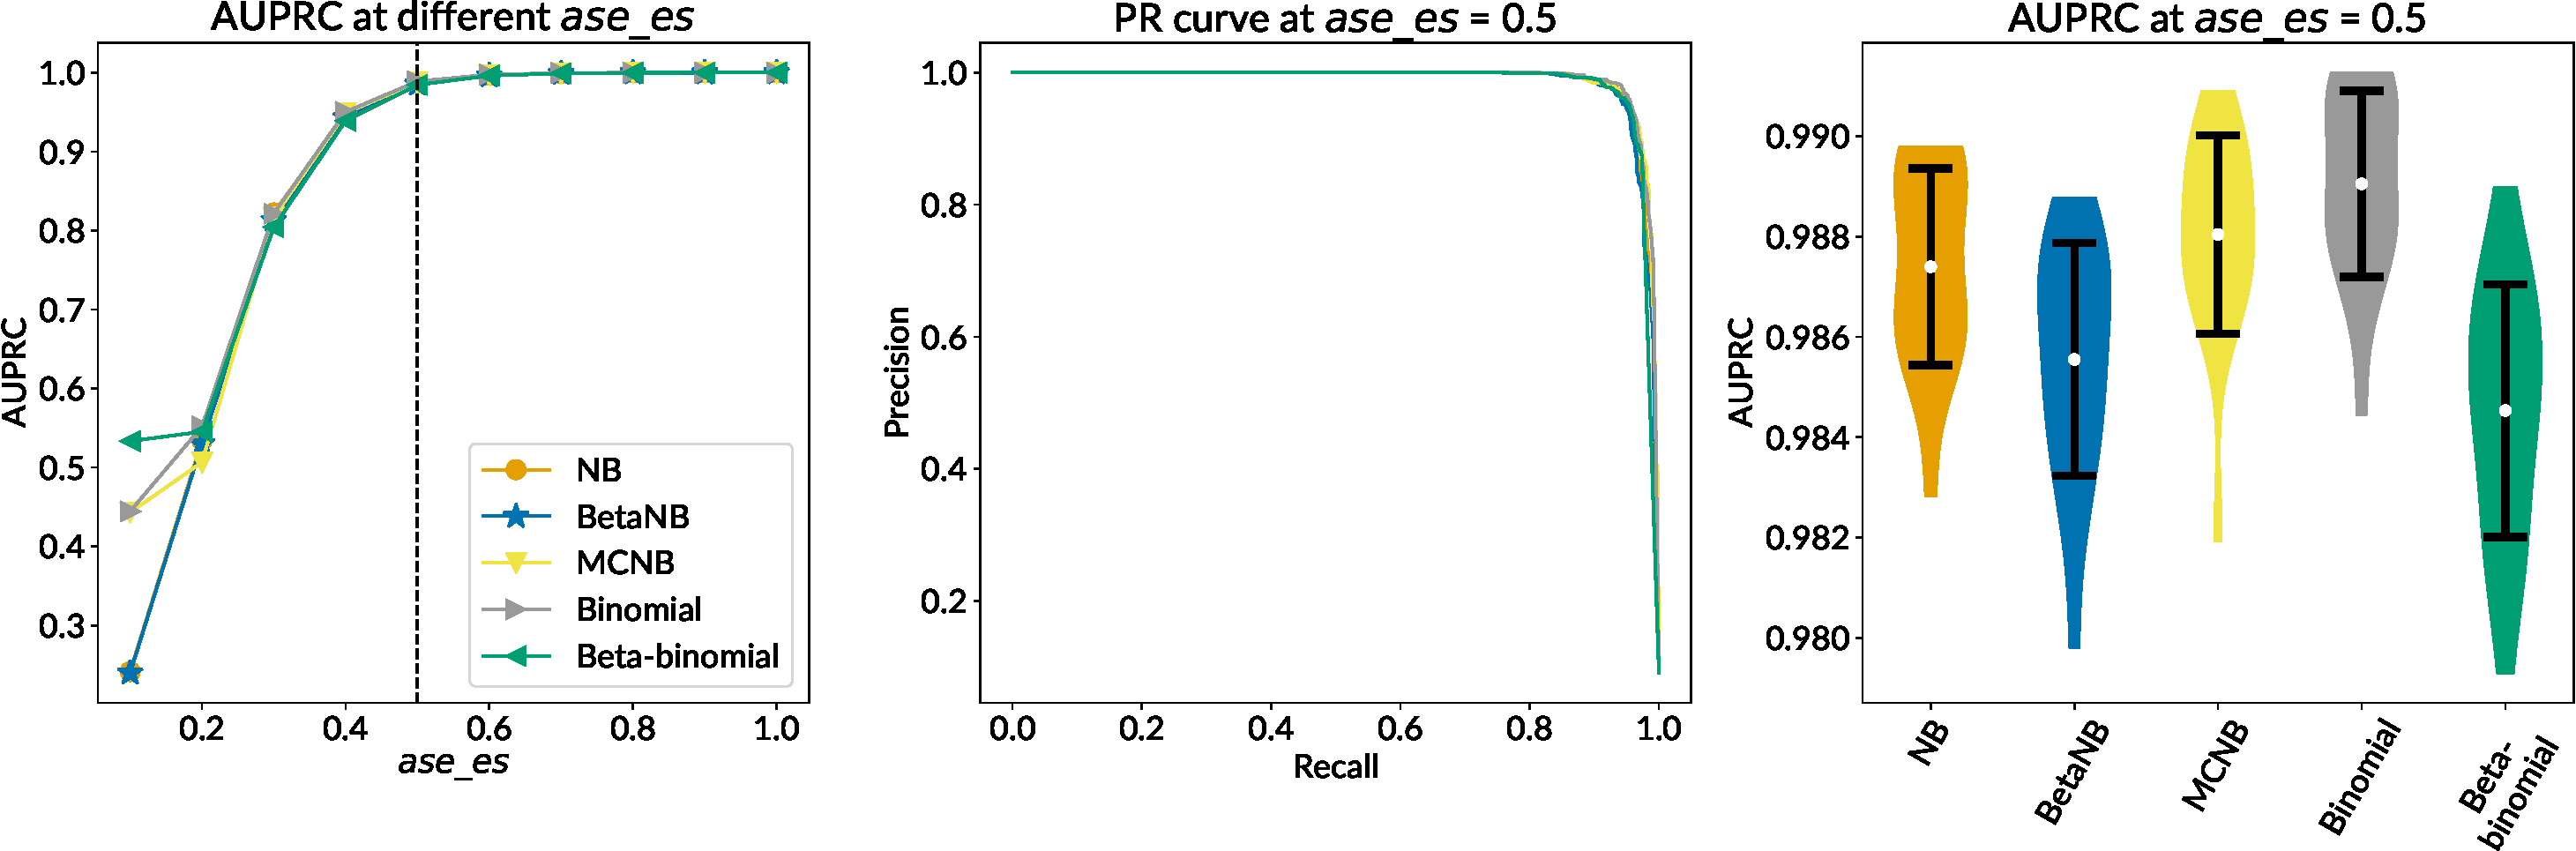
\includegraphics{figures/benchmark/B}
    				\end{adjustbox}
    \\
\raisebox{6.5em}{\Huge D} &
    				\begin{adjustbox}{max width=0.925\textwidth}
    					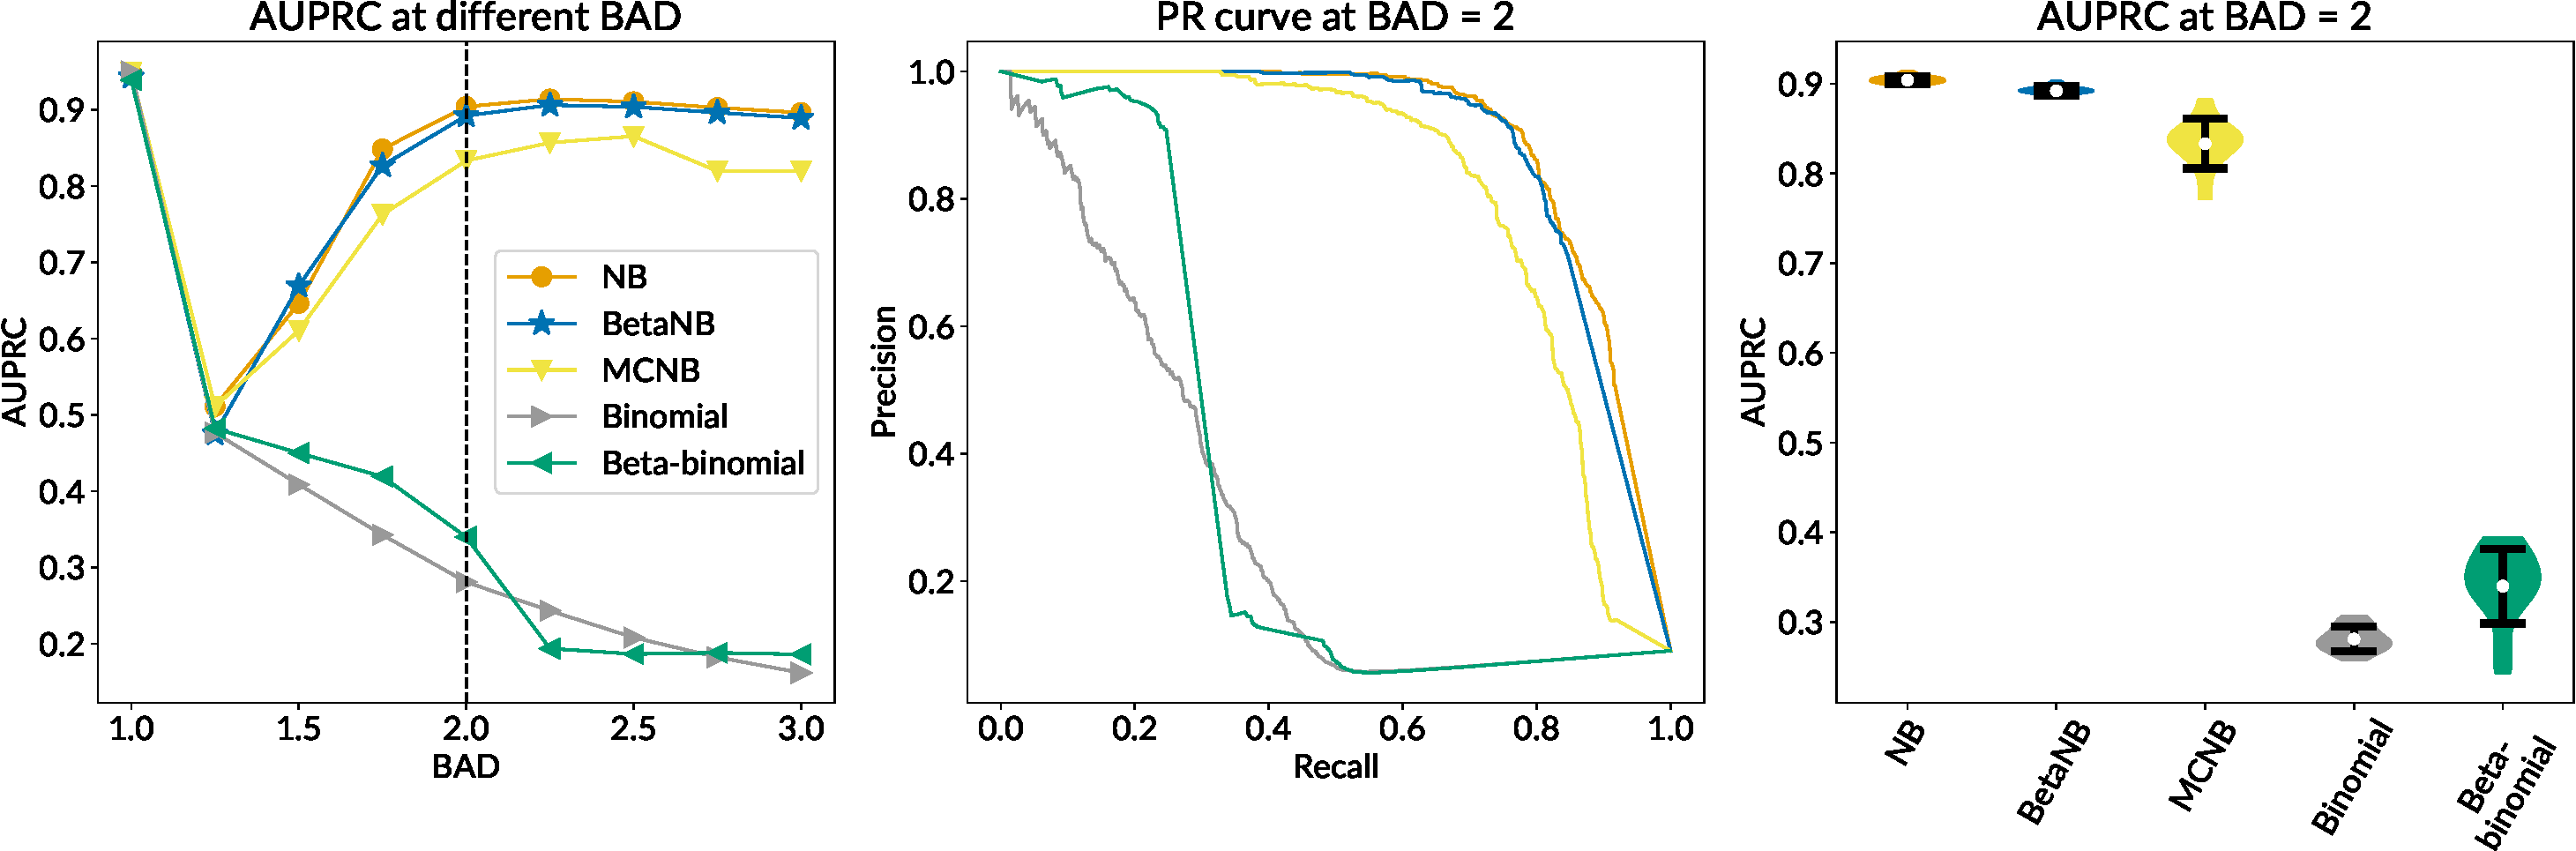
\includegraphics{figures/benchmark/D}
    				\end{adjustbox}
    \\
\raisebox{6.5em}{\Huge E} &
    				\begin{adjustbox}{max width=0.925\textwidth}
    					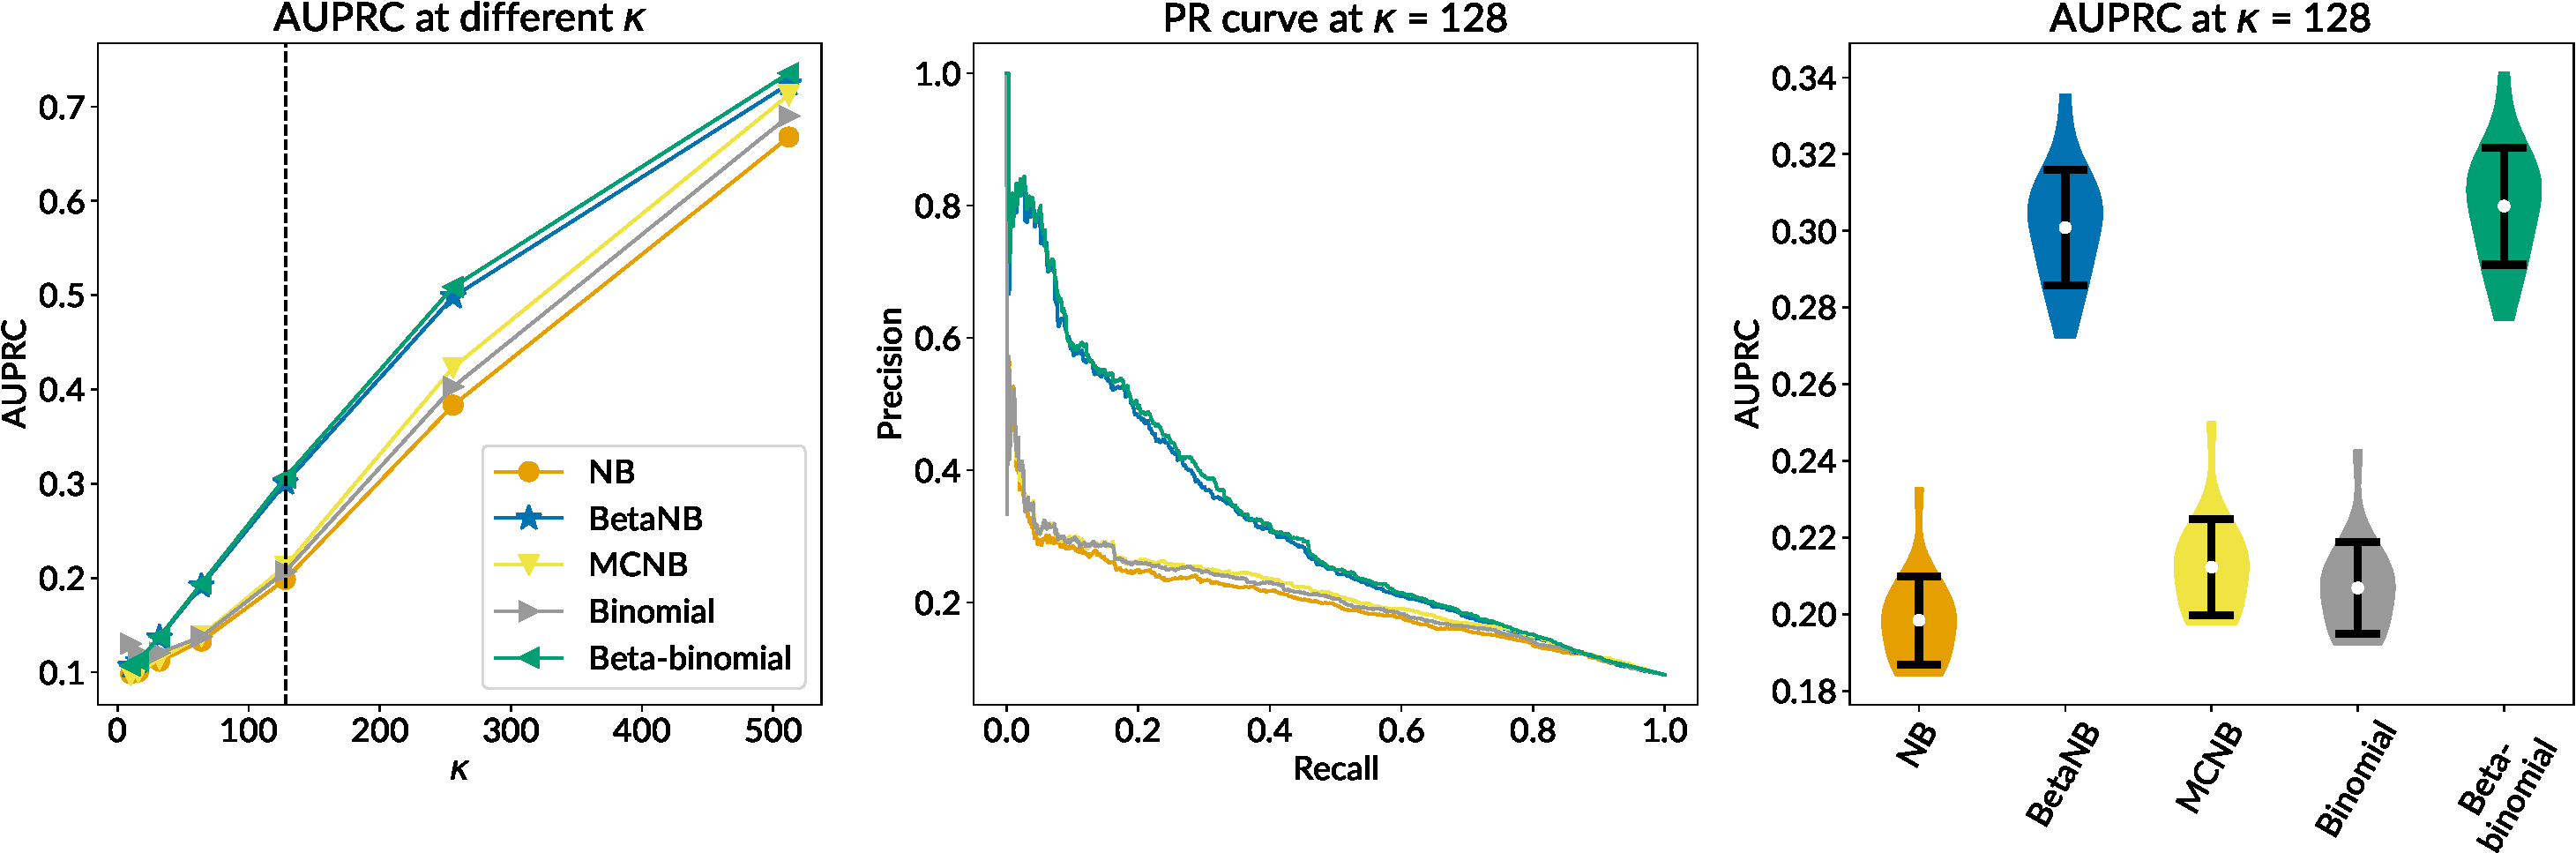
\includegraphics{figures/benchmark/E}
    				\end{adjustbox}
    \\
\raisebox{6.5em}{\Huge F} &
    				\begin{adjustbox}{max width=0.925\textwidth}
    					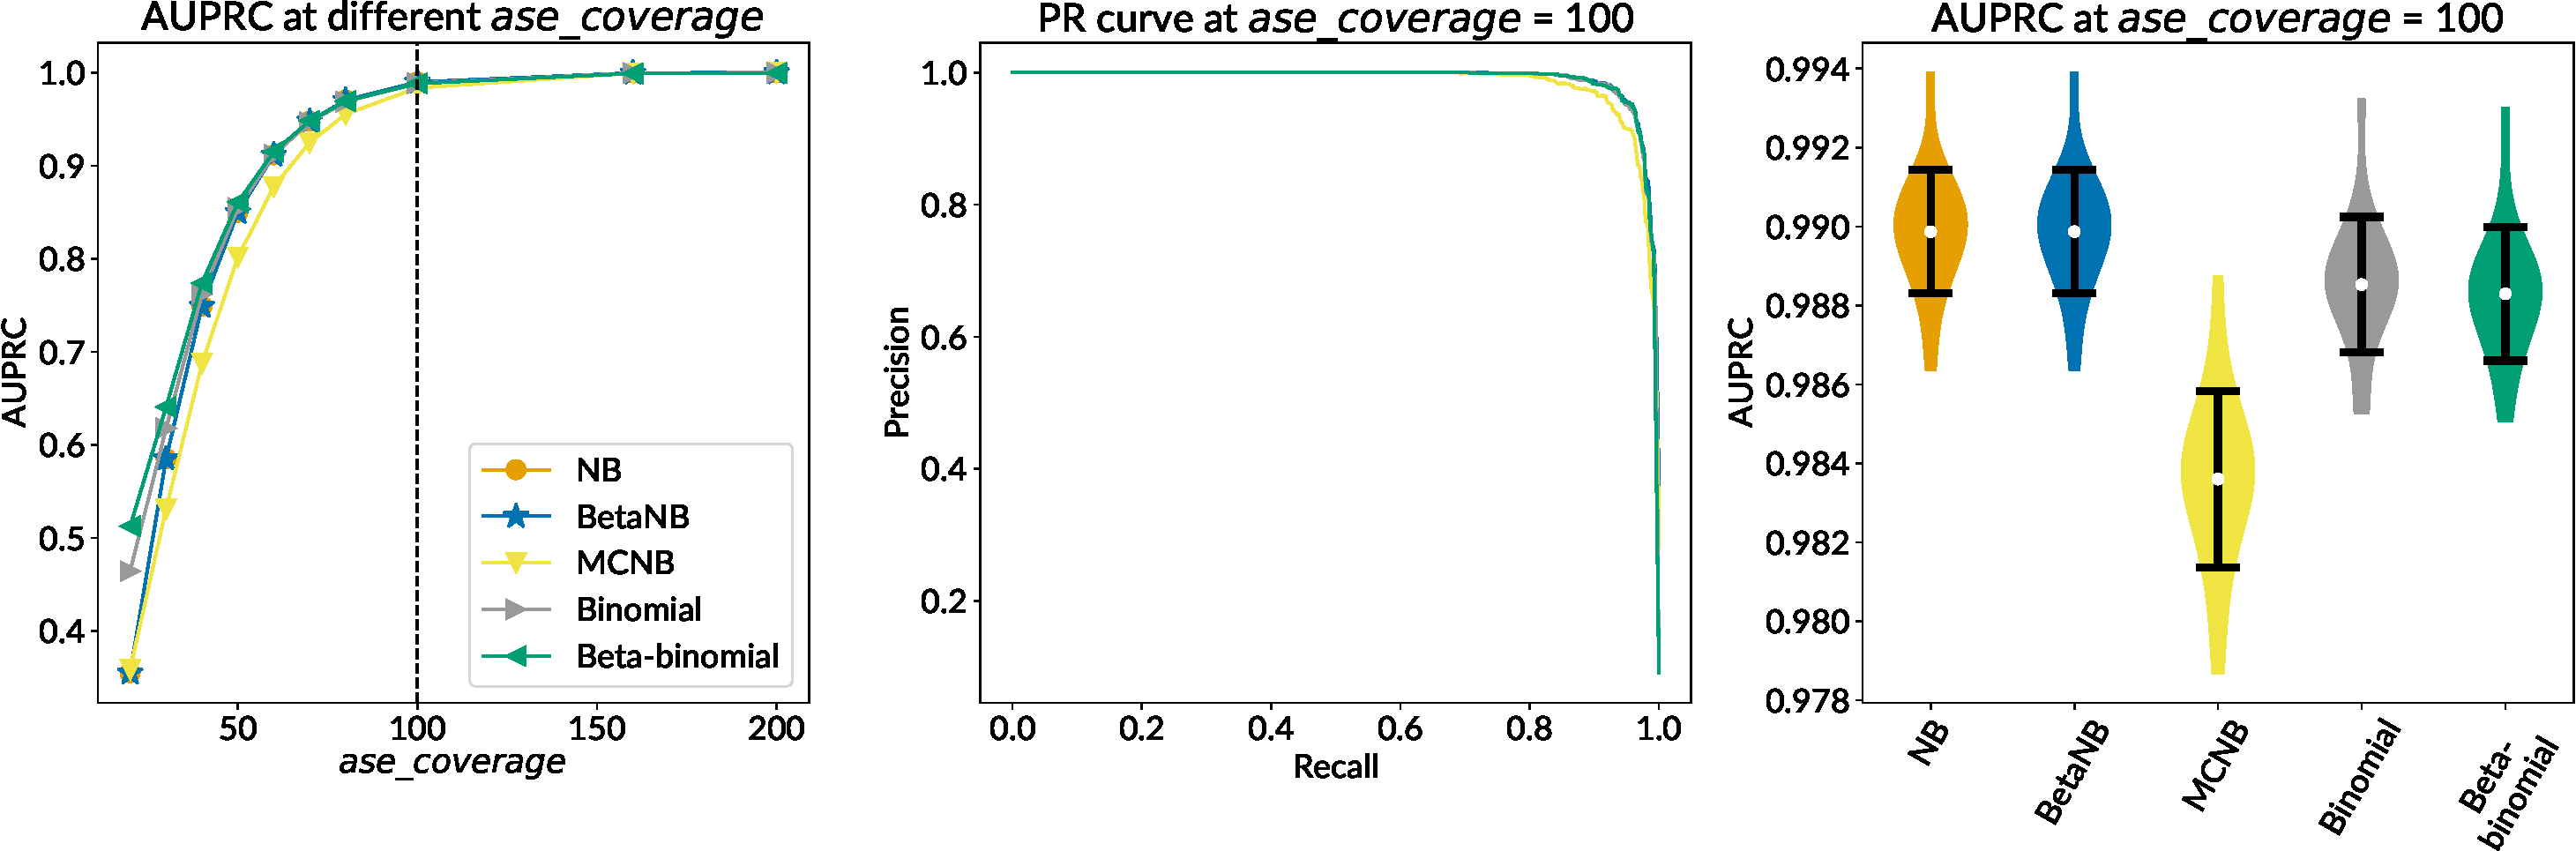
\includegraphics{figures/benchmark/F}
    				\end{adjustbox}
    \\
\raisebox{6.5em}{\Huge H} &
    				\begin{adjustbox}{max width=0.925\textwidth}
    					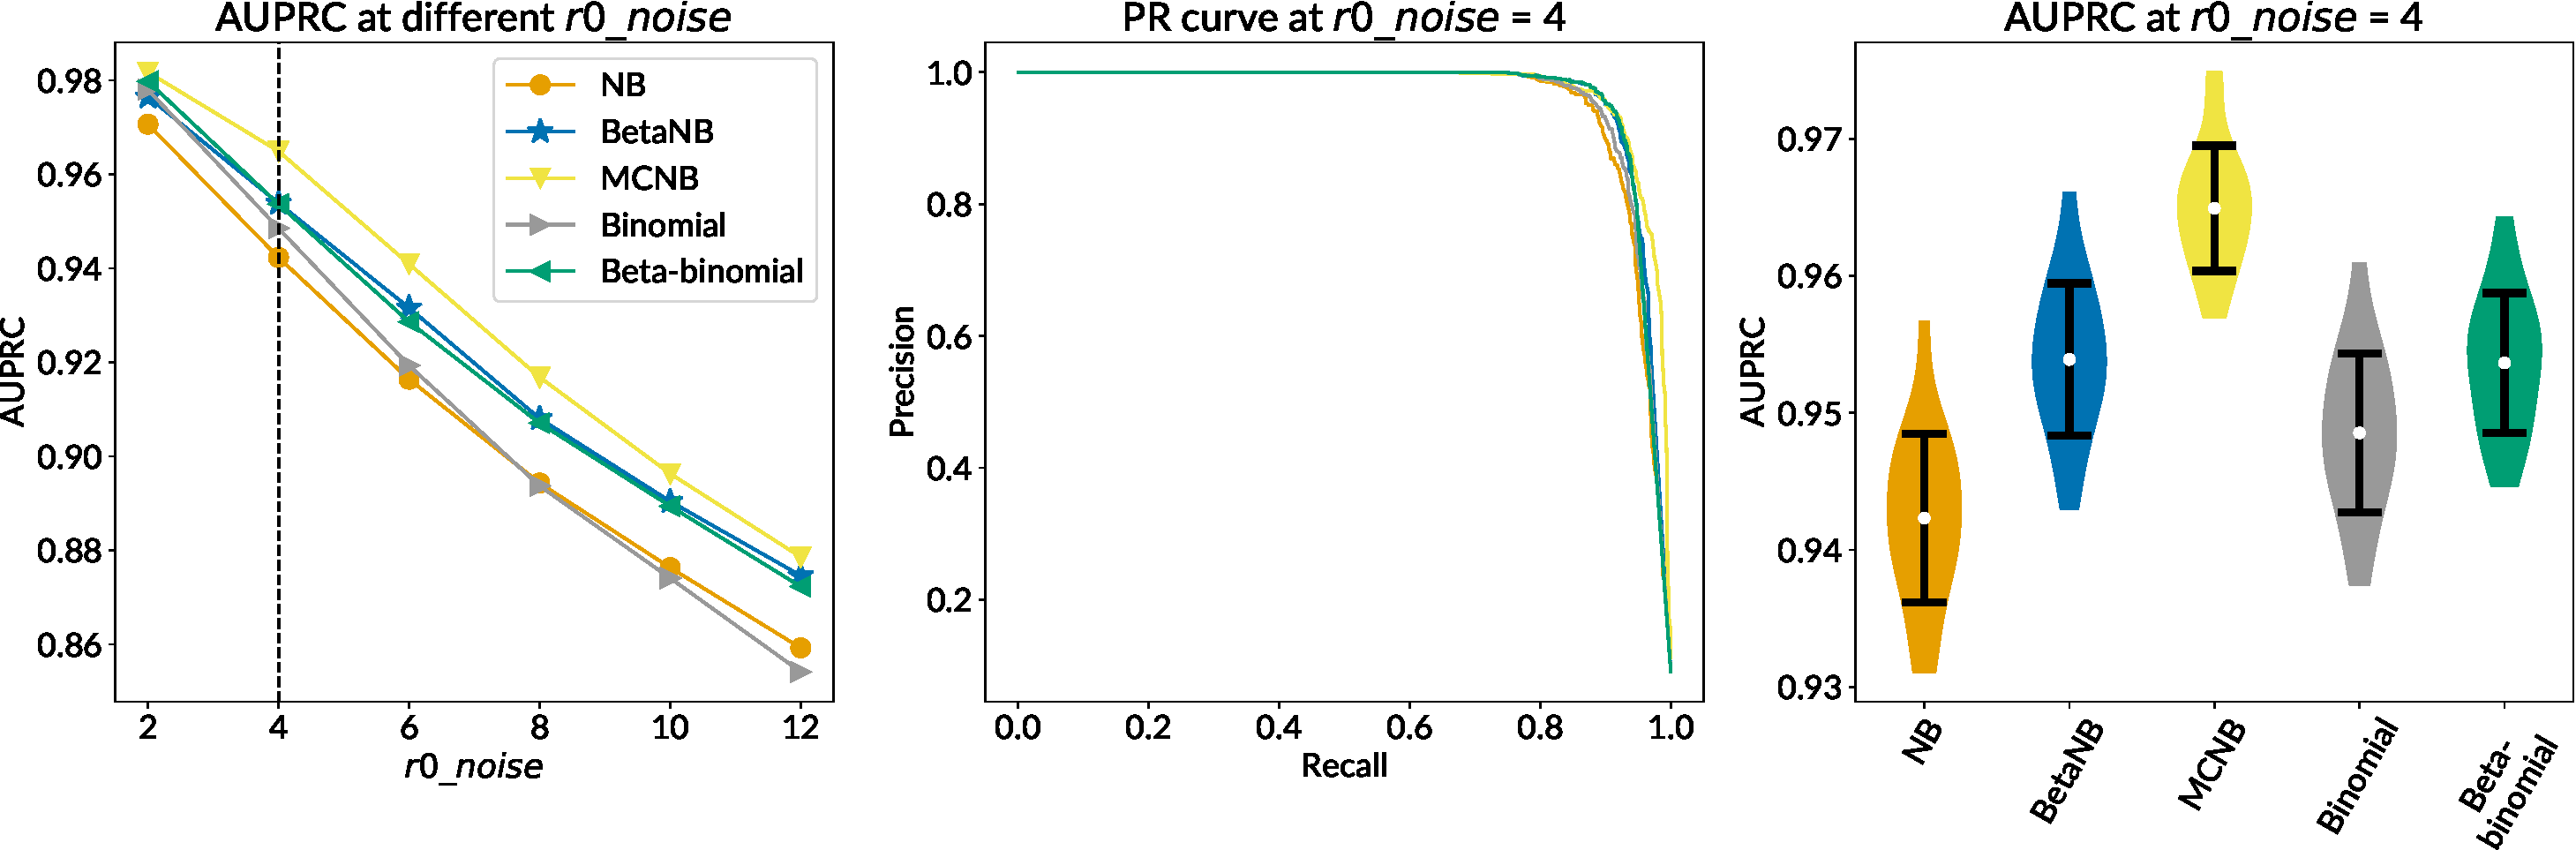
\includegraphics{figures/benchmark/H}
    				\end{adjustbox}
    \\
\raisebox{6.5em}{\Huge I} &
    				\begin{adjustbox}{max width=0.925\textwidth}
    					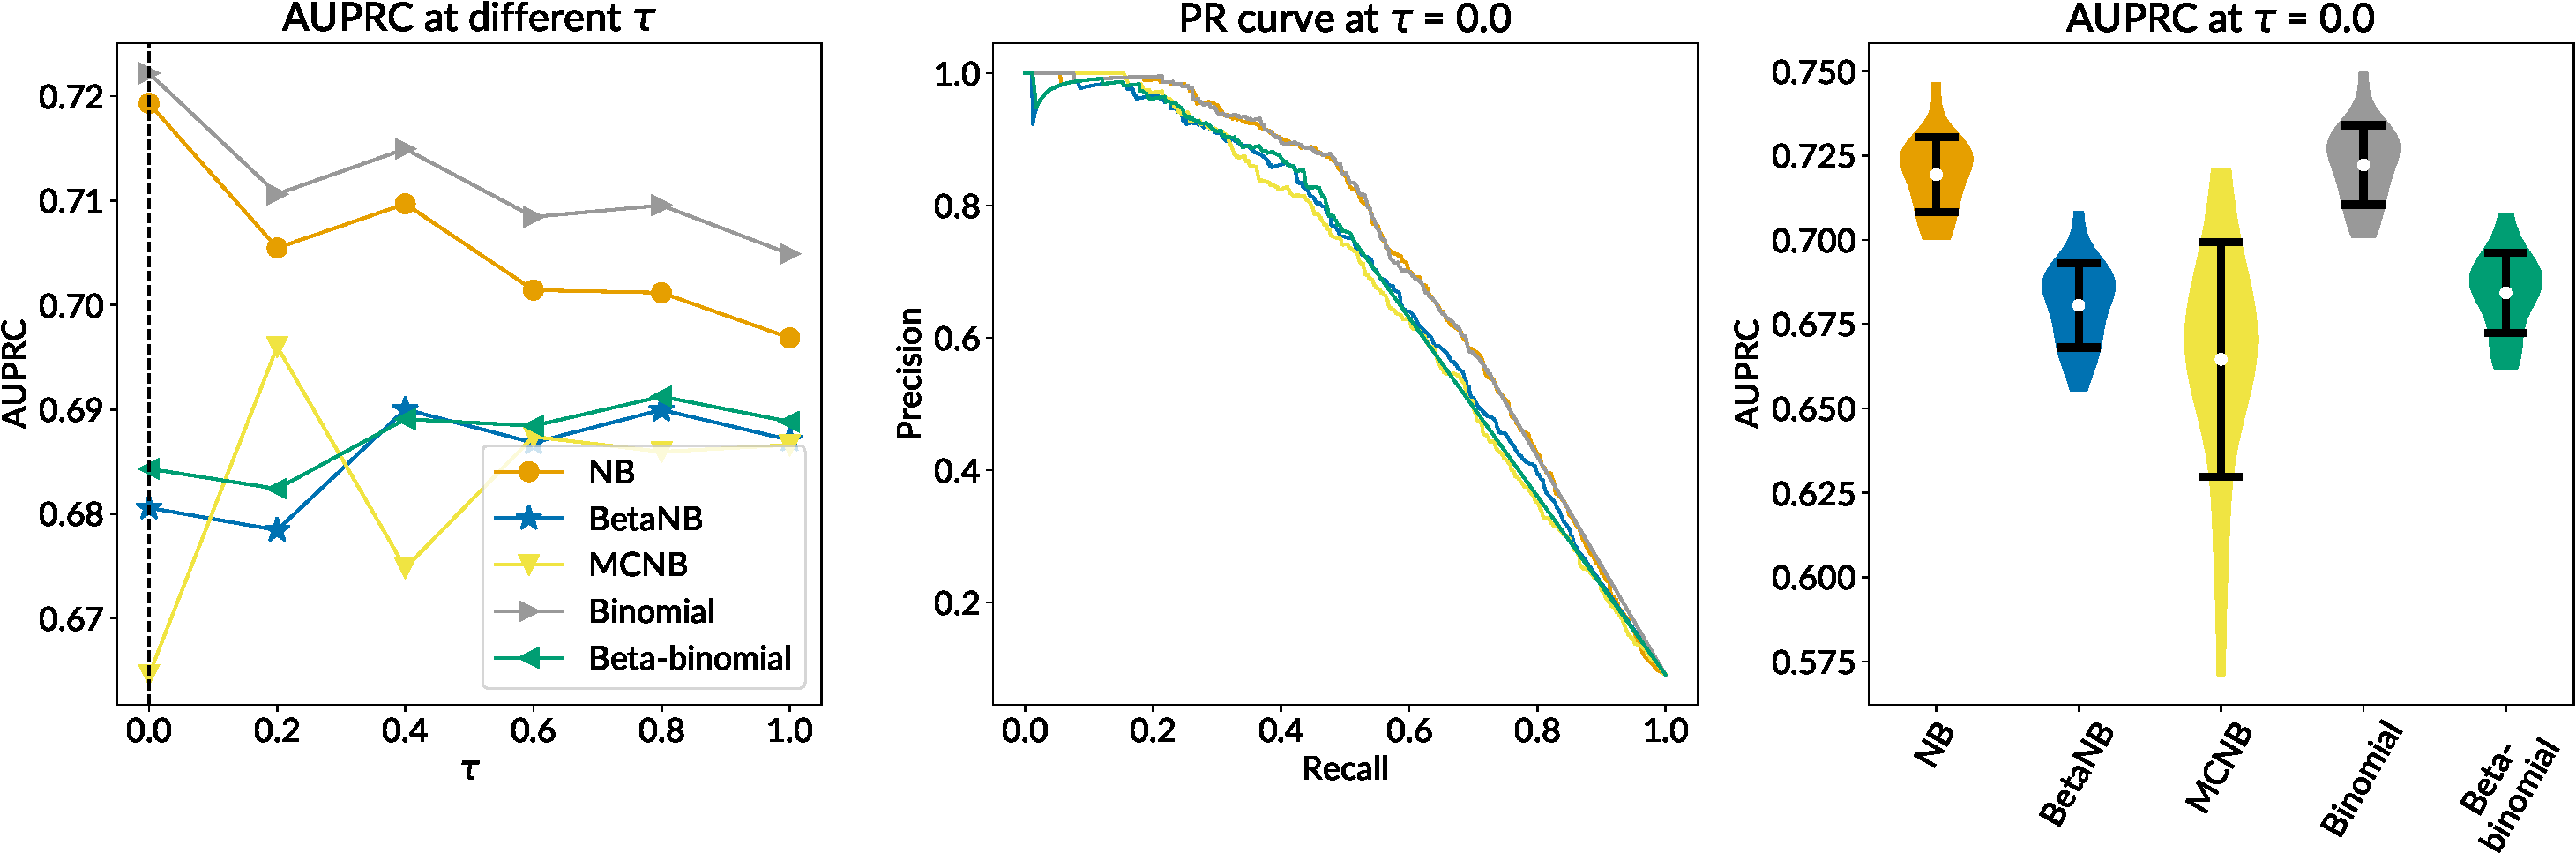
\includegraphics{figures/benchmark/I}
    				\end{adjustbox}
    \\
\raisebox{6.5em}{\Huge J} &
    				\begin{adjustbox}{max width=0.925\textwidth}
    					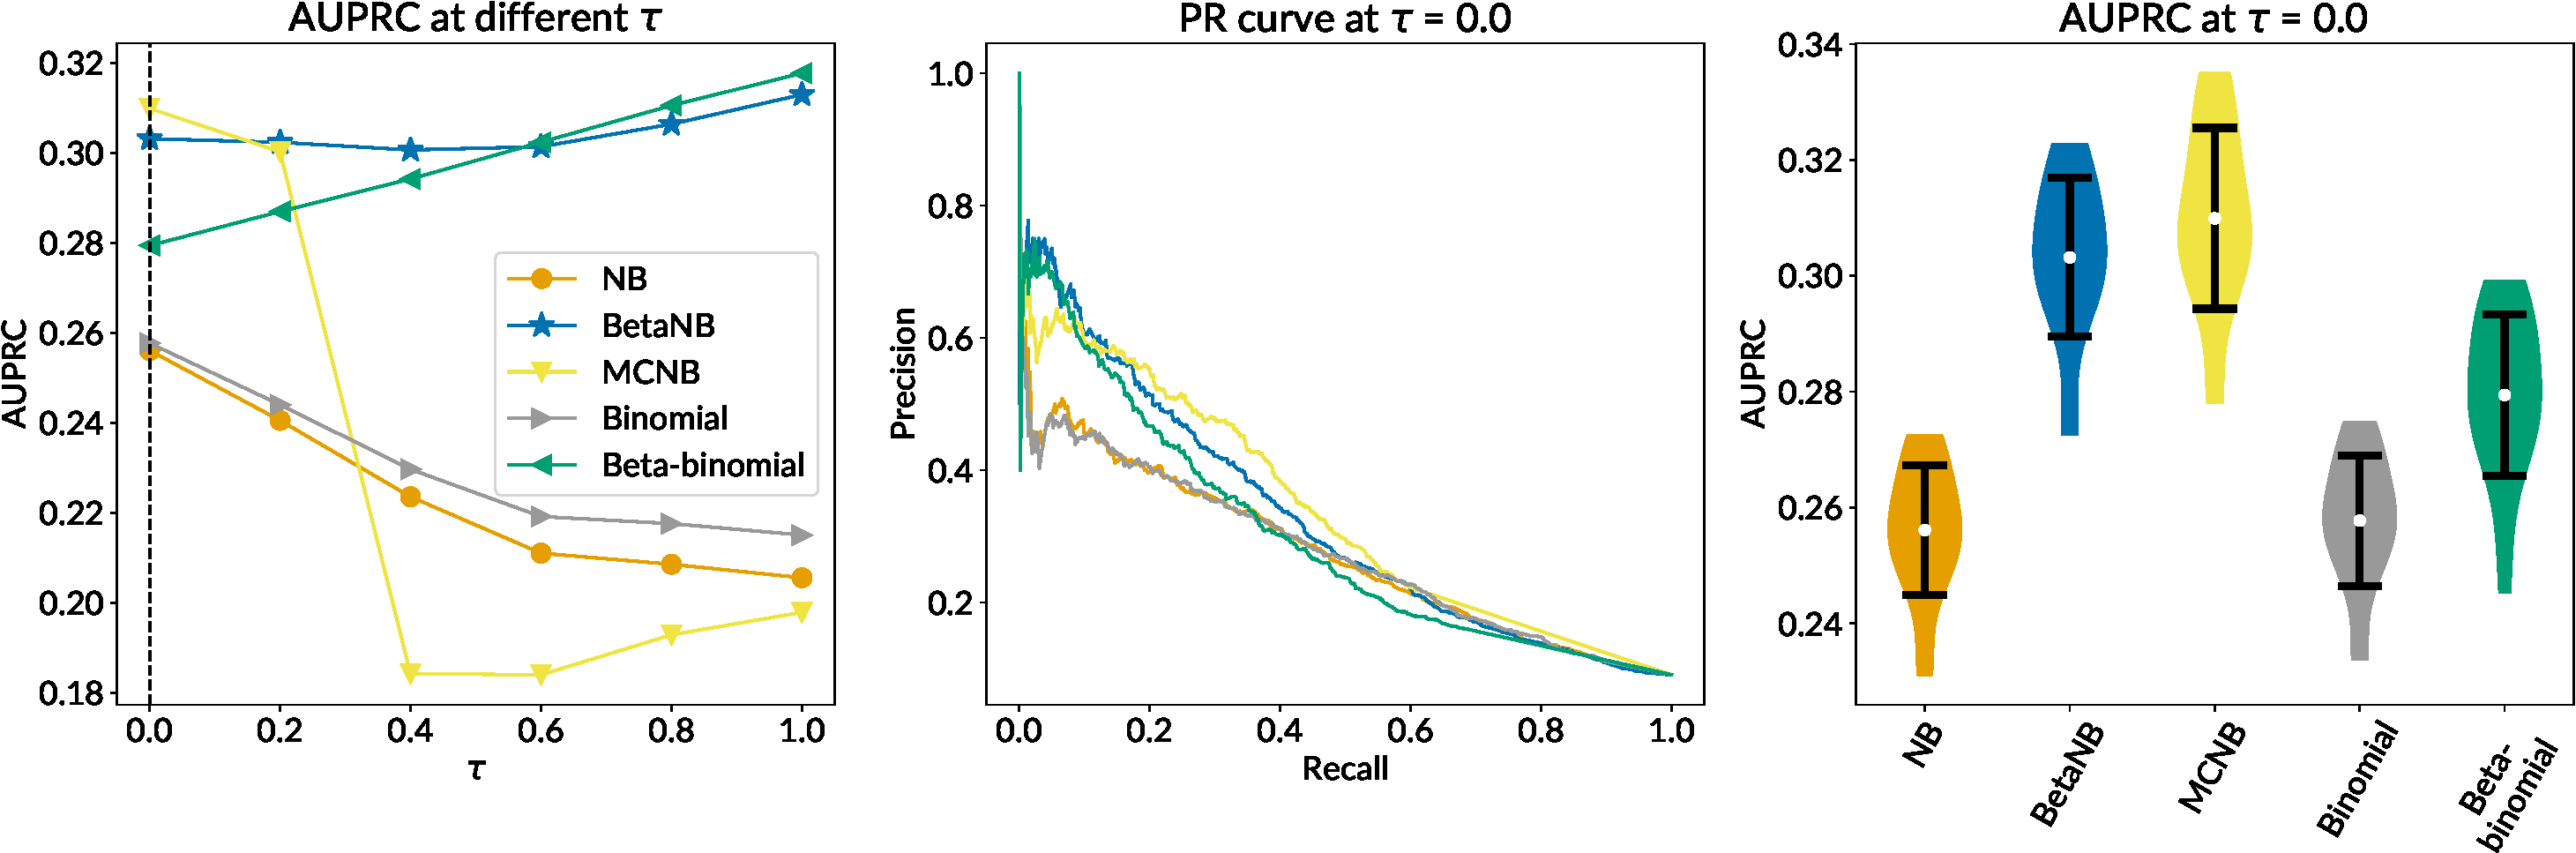
\includegraphics{figures/benchmark/J}
    				\end{adjustbox}
    \\
\raisebox{6.5em}{\Huge K} &
    				\begin{adjustbox}{max width=0.925\textwidth}
    					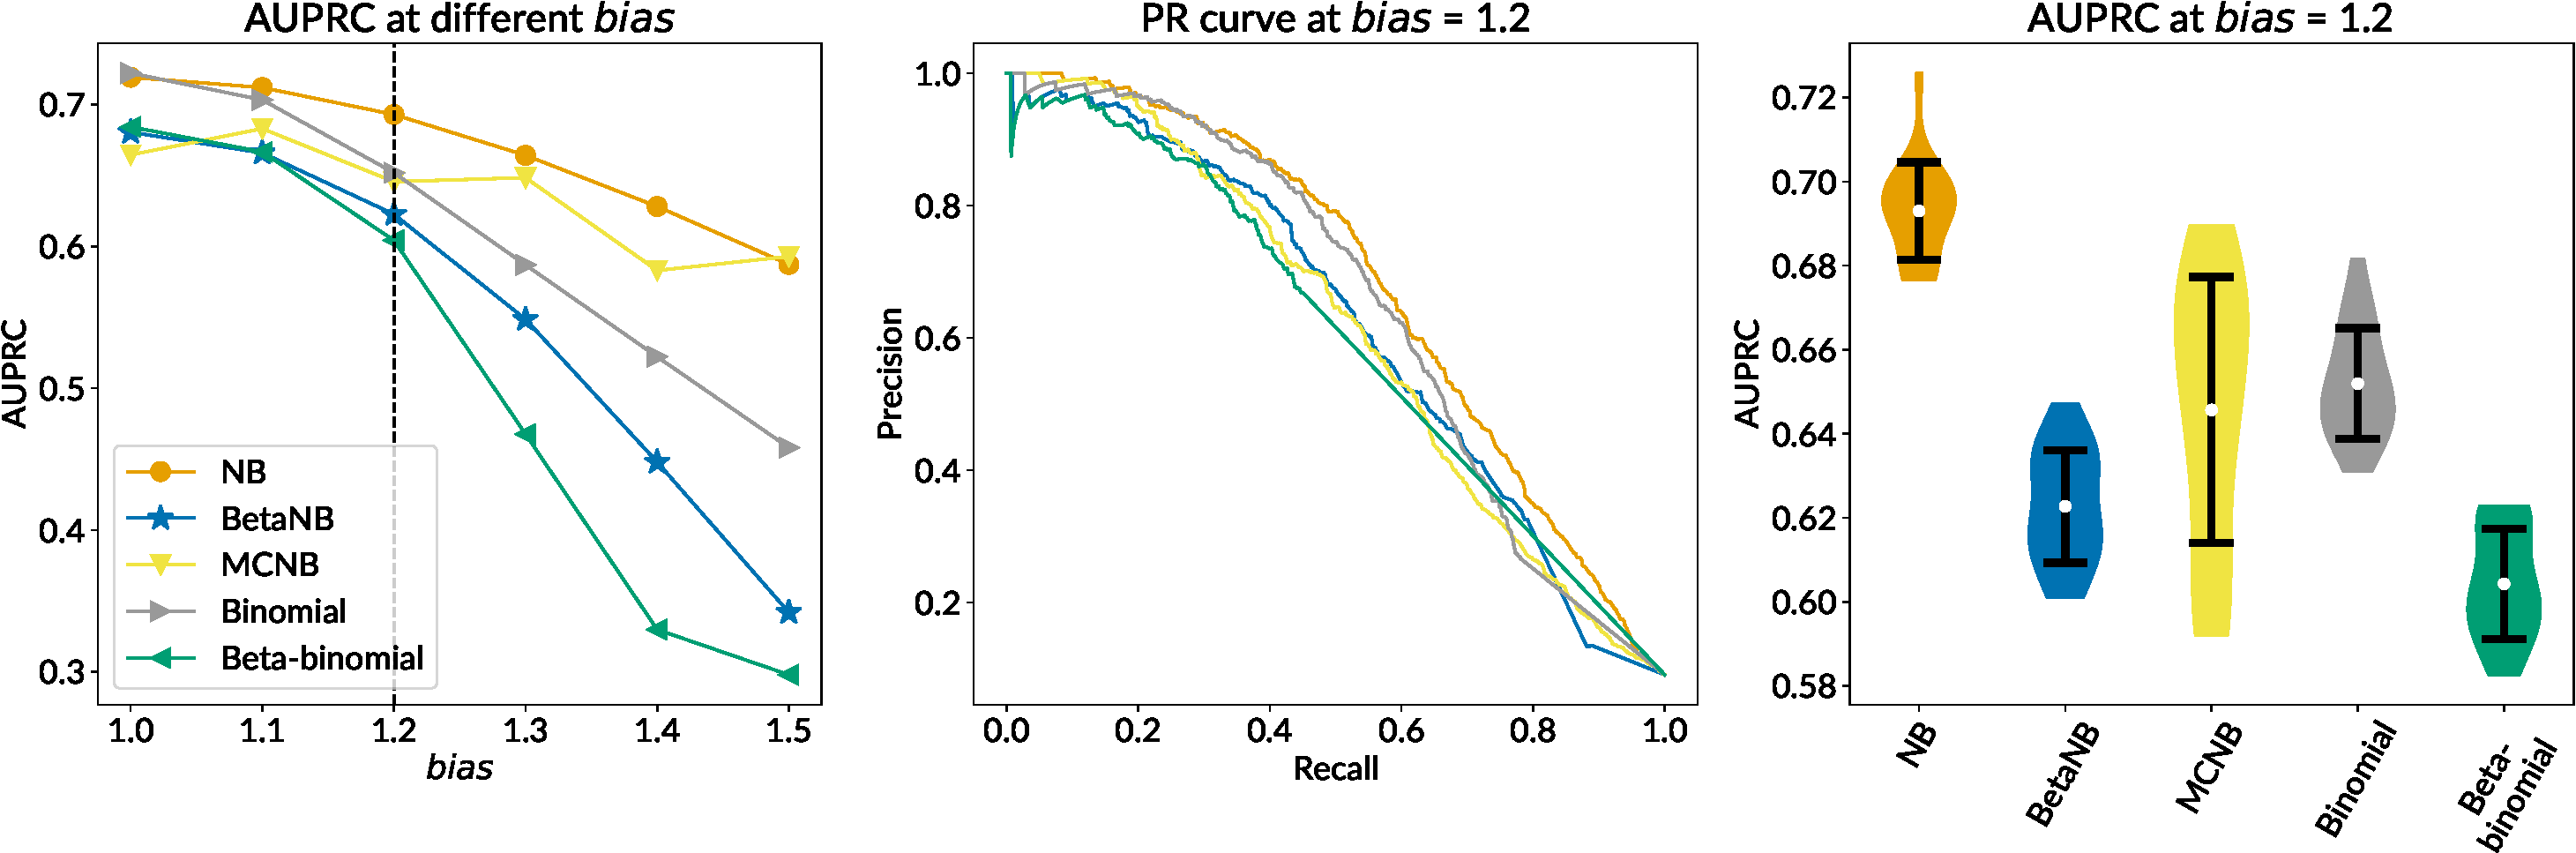
\includegraphics{figures/benchmark/K}
    				\end{adjustbox}
    \\
\raisebox{6.5em}{\Huge L} &
    				\begin{adjustbox}{max width=0.925\textwidth}
    					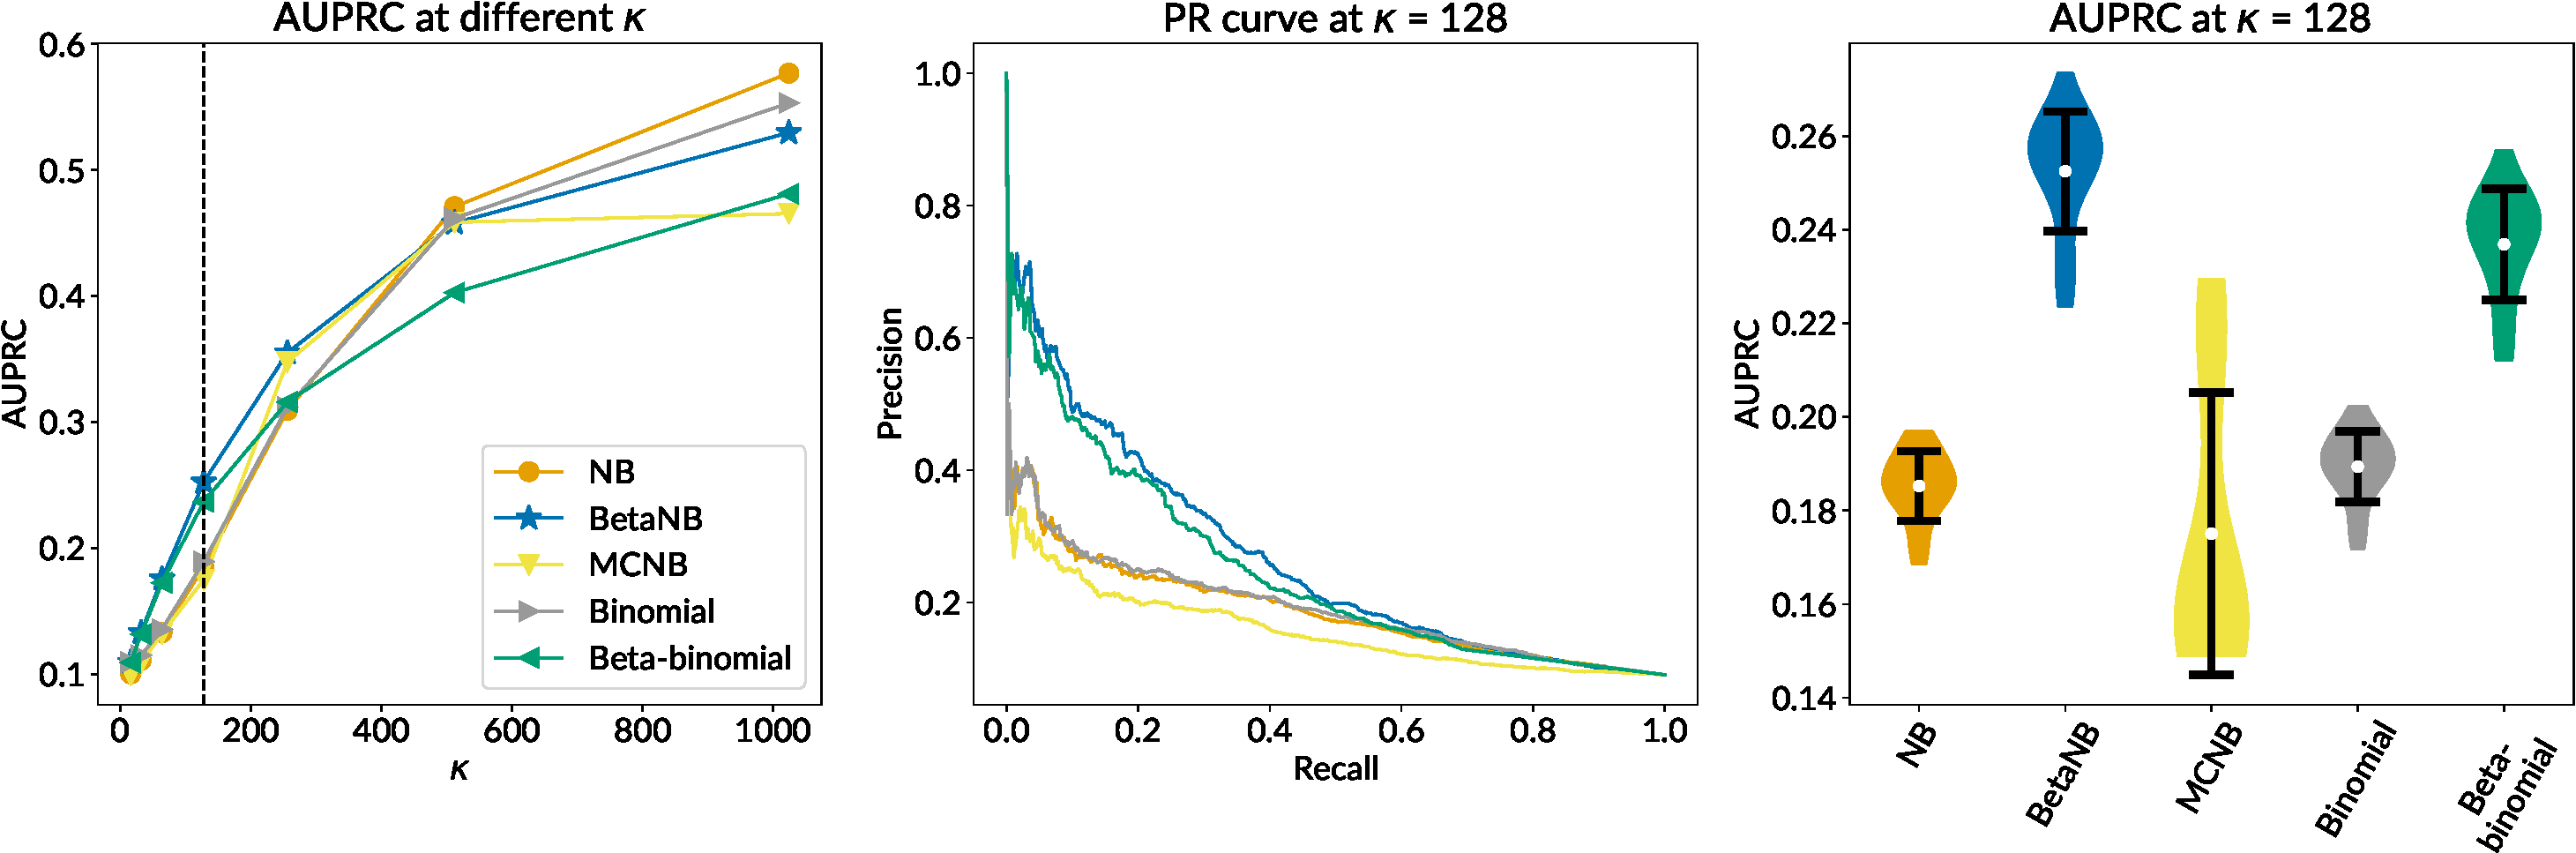
\includegraphics{figures/benchmark/L}
    				\end{adjustbox}
    
    \end{longtable}
    \captionof{figure}{PR AUC, sensitivity and specificity metrics as evaluated for various datasets. We evaluated all models present in \textbf{MIXALIME}, 
                           but for some figures only models whose performance we found relevant to the particular dataset are shown. For a complete comparison, see tables in
                           Appendix~\ref{app:benchmark_tables}. }
    \label{fig:benchmark}
    